
This and the next section will be a short recap of basic notions from measure theory and Lebesgue integration. These are inescapable subjects if one wants to understand quantum mechanics since
\ben[label=(\roman*)]
\item the spectral theorem requires the notion of (projection-valued) measures
\item the most commonly emerging separable Hilbert space in quantum mechanics is the space $L^2(\R^d)$, whose definition needs the notion of Lebesgue integral.
\een

\subsection{General measure spaces and basic results}

\bd
Let $M$ be a non-empty set. A collection $\Sigma\subseteq\mathscr{P}(M)
$ of subsets of $M$ is called a \emph{$\sigma$-algebra}\index{$\sigma$-algebra} for $M$ if the following conditions are satisfied
\ben[label=(\roman*)]
\item $M\in \Sigma$
\item if $A\in \Sigma$, then $M\setminus A \in \Sigma$
\item for any sequence $\{A_n\}_{n\in \N}$ in $\Sigma$ we have $\bigcup_{n=0}^{\infty}A_n\in\Sigma$.
\een
\ed

\br
If we relax the third condition so that it applies only to finite (rather than countable) unions, we obtain the notion of an \emph{algebra}, often called an \emph{algebra of sets} in order to distinguish it from the notion of algebra as a vector space equipped with a bilinear product, with which it has nothing to do. 
\er

\br
Note that by condition (ii) and De Morgan's laws, condition (iii) can be equivalently stated in terms of intersections rather than unions. Recall that De Morgan's laws ``interchange'' unions with intersections and vice-versa under the complement operation. That is, if $M$ is a set and $\{A_i\}_{i\in I}$ is a collection of sets, then
\bse
M \setminus \biggl(\bigcup_{\,i\in I}A_i\biggr) = \bigcap_{i\in I}(M\setminus A_i),\qquad \quad
M \setminus \biggl(\bigcap_{\,i\in I}A_i\biggr) = \bigcup_{i\in I}(M\setminus A_i).
\ese
\er

A $\sigma$-algebra is closed under countably infinite unions (by definition) but also under countably infinite intersections and finite unions and intersections.
\bp
Let $M$ be a set and let $\Sigma$ be a $\s$-algebra on $M$. Let $\{ A_n \}_{n\in \N}$ be a sequence in $\Sigma$. Then, for all $k\in \N$, we have
\ben[label=(\roman*)]
\item $\bigcup_{n=0}^k{A_n} \in \Sigma$
\item $\bigcap_{n=0}^{\infty}{A_n} \in \Sigma \ $ and $\ \bigcap_{n=0}^k{A_n} \in \Sigma$.
\een
\ep

\bq
\ben[label=(\roman*)]
\item Let the sequence $\{B_n\}_{n\in \N}$ be defined as follows:
\bse
B_n = \begin{cases} A_n \quad &\t{if }\ 0 \leq n \leq k\\
 \varnothing \quad &\t{if }\ n > k. \end{cases} 
\ese
Then, $\{B_n\}_{n\in \N}$ is a sequence in $\Sigma$, so $ \bigcup_{n=0}^{\infty}{B_n} \in \Sigma$. Hence, we have:
\bse
\bigcup_{n=0}^{\infty}{B_n} = \biggl(\bigcup_{\,n=0}^{k}{B_n}\biggr)\cup \biggl(\bigcup_{\,n=k+1}^{\infty}{\negmedspace B_n}\biggr)=\bigcup_{n=0}^k{A_n}
\ese
and thus $\bigcup_{n=0}^k{A_n} \in \Sigma$.

\item As $\{A_n\}_{n\in \N}$ is a sequence in $\Sigma$, so is $\{M\setminus A_n\}_{n\in \N}$ and hence $\bigcup_{n=0}^{\infty}{(M\setminus A_n)} \in \Sigma$. Thus, we also have
\bse
M \setminus \biggl( \bigcup_{\,n=0}^{\infty}{(M\setminus A_n)} \biggr) \in \Sigma
\ese
and since $M\setminus(M\setminus A_n)=A_n$, by De Morgan's laws, $\bigcap_{n=0}^{\infty}{A_n} \in \Sigma$. That this holds for finite intersections is shown by defining $\{B_n\}_{n\in \N}$ as above. \qedhere
\een
\eq


\bd
A \emph{measurable space} is a pair $(M,\Sigma)$ where $M$ is a set and $\Sigma$ is a $\sigma$-algebra on $M$. The elements of $\Sigma$ are called \emph{measurable subsets} of $M$.
\ed

Our goal is to assign volumes (i.e.\ measures) to subsets of a given set. Of course, we would also like this assignment to satisfy some sensible conditions. However, it turns out that one cannot sensibly assign volumes to any arbitrary collection of subsets of a given set\footnoteurl{https://en.wikipedia.org/wiki/Non-measurable_set}{}. It is necessary that the collection of subsets be a $\sigma$-algebra. In addition, just like in topology openness and closeness are not properties of subsets but properties of subsets with respect to a choice of topology, so does measurability of subsets only make sense with respect to a choice of $\sigma$-algebra. In particular, a given subset could be measurable with respect to some $\sigma$-algebra and not measurable with respect to some other $\sigma$-algebra.

\be
The pair $(M,\mathscr{P}(M))$ is a measurable space for any set $M$. Of course, just like the discrete topology is not a very useful topology, the power set $\mathscr{P}(M)$ is not a very useful $\sigma$-algebra on $M$, unless $M$ is countable.
\ee

\bd
The \emph{extended real line}\index{extended real line} is $\overline{\R} := \R \cup \{-\infty,+\infty\}$, where the symbols $-\infty$ and $+\infty$ (the latter often denoted simply by $\infty$) satisfy
\bse
\forall \, r \in \overline{\R} : \ -\infty\leq r \leq \infty
\ese
with strict inequalities if $r\in\R$.
The symbols $\pm\infty$ satisfy the following arithmetic rules
\ben[label=(\roman*)]
\item $\forall \, r\in \R : \ \pm \infty + r = r \pm \infty = \pm \infty$
\item $\forall \, r > 0 : \ r(\pm\infty)=\pm \infty\, r = \pm \infty$
\item $\forall \, r < 0 : \ r(\pm\infty)=\pm \infty\, r = \mp \infty$
\item $0(\pm\infty)=\pm \infty\, 0 = 0$.
\een
Note that expressions such as $\infty-\infty$ or $-\infty+\infty$ are not defined.
\ed
\bd
Let $(M,\Sigma)$ be a measurable space. A \emph{measure} on $(M,\Sigma)$ is a function
\bse
\mu\cl\Sigma\to[0,\infty],
\ese
where $[0,\infty]:=\{r\in\overline{\R}\mid r \geq 0\}$, such that
\ben[label=(\roman*)]
\item $\mu(\varnothing)=0$
\item for any sequence $\{A_n\}_{n\in \N}$ in $\Sigma$ with $A_i\cap A_j = \varnothing$ whenever $i\neq j$, we have
\bse
\mu\biggl(\bigcup_{\,n=0}^{\infty}A_n\biggr) = \sum_{n=0}^{\infty}\mu(A_n).
\ese
\een
\ed

A sequence $\{A_n\}_{n\in \N}$ that satisfies the condition that $A_i \cap A_j = \vn$ for all $i \neq j$ is called a \emph{pairwise disjoint} sequence.
\br
Both sides of the equation in part (ii) of the definition of measure might take the value $\infty$. There are two possible reasons why $\sum_{n=0}^{\infty}\mu(A_n)$ might be infinite. It could be that $\mu(A_n) = \infty$ for some $n\in \N$ or, alternatively, it could be that $\mu(A_n) < \infty$ for all $n \in \N$ but the sequence of partial sums $\{ \sum_{i=0}^{n}\mu(A_i)\}_{n\in\N}$, which is an increasing sequence since $\mu$ is non-negative by definition, is not bounded above.
\er

\bd
A \emph{measure space}\index{measure space} is a triple $(M,\Sigma,\mu)$ where $(M,\Sigma)$ is a measurable space and $\mu\cl\Sigma\to[0,\infty]$ is a measure on $M$.
\ed

\be \
Let $M=\N$ and $\Sigma=\mathscr{P}(\N)$. Define $\mu : \Sigma \to [0,\infty]$ by:
\bse
\mu(A) = |A|:=
\begin{cases}
n & \text{ if $A$ is a finite set with $n$ elements}\\
\infty & \text{ if $A$ is not a finite set}
\end{cases}
\ese
Then, by definition, $\mu(\vn) =0$. Moreover, if $\{A_n\}_{n\in\N}$ is a pairwise disjoint sequence in $\Sigma$ such that all but a finite number of $A_n$'s are empty and each $A_n$ has a finite number of elements, we have:
\bse
\mu \biggl( \bigcup_{\,n=0}^{\infty}A_n\biggr) = \sum_{n=0}^{\infty}\mu(A_n)
\ese
by counting elements. Otherwise, that is, if an infinite number of $A_n$'s are non-empty or if at least one $A_n$ is infinite, then
\bse
\mu \biggl( \bigcup_{\,n=0}^{\infty}A_n\biggr) = \infty = \sum_{n=0}^{\infty}\mu(A_n)
\ese
and thus, the triple $(\N,\mathscr{P}(\N),\mu)$ is a measure space. The measure $\mu$ on $(\N,\mathscr{P}(\N))$ is called \emph{counting measure} and it is the usual measure on countable measurable spaces.
\ee

\pagebreak

\bp
Let $(M,\Sigma,\mu)$ be a measure space.
\ben[label=(\roman*)]
\item If $A_0,\ldots,A_k \in \Sigma$ and $A_i \cap A_j = \varnothing$ for all $0\leq i\neq j\leq k$, then:
\bse
\mu \biggl( \bigcup_{\,n=0}^{k}A_n\biggr) = \sum_{n=0}^{k}\mu(A_n)
\ese
\item If $A,B\in \Sigma$ and $A \subseteq B$, then $\mu(A) \leq \mu(B)$
\item If $A,B \in \Sigma$, $A \subseteq B$ and $\mu(A)<\infty$, then $ \mu(B\setminus A)=\mu(B)-\mu(A)$.
\een
\ep

\bq
\ben[label=(\roman*)]
\item Let $A_n=\varnothing$ for all $n>k$. Then, $\{A_n\}_{n\in\N}$ is a pairwise disjoint sequence in $\Sigma$ and hence, we have:
\bse
\mu \biggl( \bigcup_{\,n=0}^{k}A_n\biggr) =\mu \biggl( \bigcup_{\,n=0}^{\infty}A_n\biggr) = \sum_{n=0}^{\infty}\mu(A_n)= \sum_{n=0}^{k}\mu(A_n).
\ese
\item We have $B=A\cup (B\setminus A)$ and $A\cap (B\setminus A)=\varnothing$. Hence, by part (i),
\bse
\mu(B)= \mu(A\cup (B\setminus A))=\mu(A)+\mu ( B\setminus A),
\ese
and since $\mu ( B\setminus A)\geq 0$, we have $ \mu(A) \leq \mu(B)$.
\item By decomposing $B$ as above and rearranging, we immediately get
\bse
\mu(B\setminus A)=\mu(B)-\mu(A).
\ese
Note, however, that this only makes sense if $\mu(A)<\infty$, for otherwise we must also have $\mu(B)=\infty$ by part (ii), and then $\mu(B)-\mu(A)$ would not be defined.
\qedhere
\een 
\eq

\bp
Let $(M,\Sigma,\mu)$ be a measure space and let $\{A_n\}_{n\in \N}$ be a sequence in $\Sigma$.
\ben[label=(\roman*)]
\item If $\{A_n\}_{n\in \N}$ is increasing, i.e.\ $A_n\subseteq A_{n+1}$ for all $n \in \N$, then
\bse
\mu \biggl( \bigcup_{\,n=0}^{\infty}A_n\biggr) = \lim_{n \to \infty} \mu(A_n).
\ese
\item If $\mu(A_0)<\infty$ and $\{A_n\}_{n\in \N}$ is decreasing, i.e.\ $ A_{n+1}\subseteq A_n$ for all $n \in \N$, then
\bse
\mu \biggl(  \bigcap_{\,n=0}^{\infty}E_n\biggr) = \lim_{n \to \infty} \mu(A_n).
\ese
\een
\ep
We say that $\mu$ is (i) \emph{continuous from below} and (ii) \emph{continuous from above}.

\bq
\ben[label=(\roman*)]
\item Define $B_0:=A_0$ and $B_n := A_n\setminus A_{n-1}$. Then, $\{ B_n \}_{n\in\N}$ is a pairwise disjoint sequence in $\Sigma$ such that \bse
\bigcup_{i=0}^n B_i = A_n\qquad \text{ and }\qquad \bigcup_{n=0}^{\infty} A_n=\bigcup_{n=0}^{\infty} B_n.
\ese

Hence, we have
\bi{rCl}
\mu \biggl(\bigcup_{\,n=0}^{\infty}A_n\biggr) &=&  \mu \biggl(\bigcup_{\,n=0}^{\infty}B_n\biggr)\\
&=& \sum_{n=0}^{\infty}\mu(B_n) \\
&=& \lim_{n \to \infty}\sum_{i=0}^n \mu(B_i)\\
&=& \lim_{n \to \infty}\mu \biggl(\bigcup_{\,i=0}^{n}B_n\biggr) \\
&=&  \lim_{n \to \infty} \mu(A_n) .
\ei

\item Define $B_n := A_0\setminus A_n$. Then, $B_n \subseteq B_{n+1}$ for all $n \in \N$ and thus, by part (i), we have
\bi{rCl}
\mu \biggl( \bigcup_{\,n=0}^{\infty}B_n\biggr) & = &  \lim_{n \to \infty} \mu(B_n) \\
& = & \lim_{n \to \infty} ( \mu(A_0)-\mu(A_n))\\[2pt]
& = & \mu(A_0)-\lim_{n \to \infty} \mu(A_n).
\ei
Note that, by definition of $B_n$, we have
\bse
\bigcup_{n=0}^{\infty}B_n = A_0 \setminus \bigcap_{\,n=0}^{\infty}A_n.
\ese
Since $\mu(A_0)<\infty$, it follows from the previous proposition that
\bi{rCl}
\mu(A_0)-\mu \biggl(\bigcap_{\,n=0}^{\infty}A_n\biggr) &= & \mu \biggl( A_0 \setminus \bigcap_{n=0}^{\infty}A_n\biggr) \\
&=& \mu \biggl(\bigcup_{\,n=0}^{\infty}B_n\biggr)\\
&=&  \mu(A_0)-\lim_{n \to \infty} \mu(A_n).
\ei
Therefore, we have 
\bse
\mu \biggl( \bigcap_{n=1}^{\infty}A_n\biggr) = \lim_{n \to \infty} \mu(A_n). \qedhere
\ese
\een
\eq

\br
Note that the result in the second part of this proposition need not be true if $\mu(A_0)=\infty$. For example, consider $(\N,\mathscr{P}(\N),\mu)$, where $\mu$ is the counting measure on $(\N,\mathscr{P}(\N))$. If $A_n = \{n, n+1, n+2, \ldots\}$, then $\{A_n\}_{n\in\N}$ is a decreasing sequence. Since $\mu(A_n) = \infty$ for all $n \in \N$, we have $\displaystyle \lim_{n \to \infty} \mu(A_n) = \infty$. On the other hand, $ \bigcap_{n=0}^{\infty}A_n = \varnothing$ and thus $\mu(\bigcap_{n=0}^{\infty}A_n) =0$.
\er

\bp
Let $(M,\Sigma,\mu)$ be a measure space. Then, $\mu$ is countably sub-additive. That is, for any sequence $\{A_n\}_{n\in\N}$ in $\Sigma$, we have
\bse
\mu\biggl(\bigcup_{\,n=0}^{\infty}A_n\biggr)\leq \sum_{n=0}^{\infty}\mu(A_n).
\ese
\ep


\bq
\ben[label=(\alph*)]
\item First, we show that $\mu(A\cup B)\leq \mu(A)+\mu(B)$ for any $A,B\in\Sigma$. Note that, for any pair of sets $A$ and $B$, the sets $A\setminus B$, $B\setminus A$ and $A\cap B$ are pairwise disjoint and their union is $A\cup B$.
\begin{center}
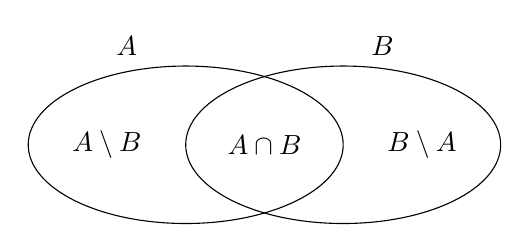
\begin{tikzpicture}[scale=0.5]
\draw (-3.5,1.5) ellipse (4 and 2);
\draw (0.5,1.5) ellipse (4 and 2);
\node at (-5.5,1.5) {$A\setminus B$};
\node at (-1.5,1.5) {$A\cap B$};
\node at (2.5,1.5) {$B\setminus A$};
\node at (-5,4) {$A$};
\node at (1.5,4) {$B$};
\end{tikzpicture}
\end{center}
By writing $A = (A\setminus B ) \cup (A\cap B)$ and $B = (B\setminus A ) \cup (A\cap B)$ and using the additivity and positivity of $\mu$, we have
\bi{rCl}
\mu(A)+\mu(B)& = &\mu((A\setminus B ) \cup (A\cap B))+\mu((B\setminus A ) \cup (A\cap B))\\
& = &\mu(A\setminus B ) + 2\mu(A\cap B)+\mu(B\setminus A )\\
& = &\mu(A\cup B ) + \mu(A\cap B)\\
& \geq & \mu(A\cup B ).
\ei
\item We now extend this to finite unions by induction. Let $\{A_n\}_{n\in\N}$ be a sequence in $\Sigma$ and suppose that
\bse
\mu\biggl(\bigcup_{\,i=0}^{n}A_i\biggr)\leq \sum_{i=0}^{n}\mu(A_i)
\ese
for some $n\in \N$. Then, by part (a), we have
\bi{rCl}
\mu\biggl(\bigcup_{\,i=0}^{\,n+1}A_i\biggr) & = & \mu\biggl(A_{n+1}\cup\bigcup_{i=0}^{n}A_i\biggr)\\
& \leq &\mu (A_{n+1})+\mu\biggl(\bigcup_{\,i=0}^{n}A_i\biggr)\\
& \leq &\mu (A_{n+1})+\sum_{i=0}^{n}\mu(A_i)\\
& = & \sum_{i=0}^{n+1}\mu(A_i).
\ei
Hence, by induction on $n$ with base case $n=1$ and noting that the case $n=0$ is trivial (it reduces to $\mu(A_0)=\mu(A_0)$), we have
\bse
\forall \, n \in \N : \ \mu\biggl(\bigcup_{\,i=0}^{n}A_i\biggr)\leq \sum_{i=0}^{n}\mu(A_i).
\ese
\item Let $\{A_n\}_{n\in\N}$ be a sequence in $\Sigma$. Define $B_n:=\bigcup_{i=0}^nA_n$. Then, $\{B_n\}_{n\in\N}$ is an increasing sequence in $\Sigma$. Hence, by continuity from above of $\mu$, we have
\bi{rCl}
\mu\biggl(\bigcup_{\,n=0}^{\infty}A_n\biggr) &=& \mu\biggl(\bigcup_{\,n=0}^{\infty}B_n\biggr)\\
& = & \lim_{n\to\infty}\mu(B_n)\\
& = & \lim_{n\to\infty}\mu\biggl(\bigcup_{\,i=0}^{n}A_i\biggr)\\
& \leq & \lim_{n\to\infty}\sum_{i=0}^n\mu(A_i)\\
& = & \sum_{i=0}^\infty\mu(A_i)
\ei
which is what we wanted. \qedhere
\een
\eq

\bd
Let $(M,\Sigma,\mu)$ be a measure space. The measure $\mu$ is said to be \emph{finite}\index{finite measure} if there exists a sequence $\{A_n\}_{n\in\N}$ in $\Sigma$ such that $\bigcup_{n=0}^{\infty}A_n=M$ and
\bse
\forall \, n \in \N : \ \mu(A_n)<\infty.
\ese
\ed

\be
The counting measure on $(\N,\mathscr{P}(\N))$ is finite. To see this, define $A_n:=\{n\}$. Then, clearly $\bigcup_{n=0}^{\infty}A_n=\N$ and $\mu(A_n)=|\{n\}|=1<\infty$ for all $n\in \N$.
\ee



\subsection[\texorpdfstring{Borel $\sigma$-algebras}{Borel \textsigma-algebras}]{Borel $\sigma$-algebras}

We have already remarked the parallel between topologies and $\sigma$-algebras. A further similarity stems from the fact that, just like for topologies, interesting $\sigma$-algebras are hardly ever given explicitly, except in some simple cases. In general, they are defined implicitly by some membership condition.

\bp
Let $M$ be a set and let $\{ \Sigma_i : i \in I\}$ be a collection of $\s$-algebras on $M$. Define the set
\bse
\Sigma :=\bigcap_{i\in I}\Sigma_i = \{ A \in \mathscr{P}(M) \mid A \in \Sigma_i, \forall \, i \in I \}.
\ese
Then, $\Sigma$ is a $\s$-algebra on $M$.
\ep
\bq
We simply check that $\Sigma$ satisfies the defining properties of a $\sigma$-algebra.
\ben[label=(\roman*)]
\item We have $M \in \Sigma_i$ for all $i \in I$ and hence $ M \in \Sigma$.  
\item Let $A \in \Sigma$. Then, $A \in \Sigma_i$ for all $i \in I$
and, since each $\Sigma_i$ is a $\s$-algebra, we also have $M\setminus A \in \Sigma_i$ for all $i\in I$. Hence, $M\setminus A \in \Sigma$.
\item Let $\{A_n\}_{n\in\N}$ be a sequence in $\Sigma$. Then, $\{A_n\}_{n\in\N}$ is a sequence in each $\Sigma_i$. Thus,
\bse
\forall \, i\in I : \ \bigcup_{n=0}^{\infty}{A_n} \in \Sigma_i.
\ese
Hence, we also have $\bigcup_{n=0}^{\infty}{A_n} \in \Sigma$. \qedhere
\een
\eq

\bd
Let $M$ be a set and let $\mathcal{E}\subseteq\mathscr{P}(M)$ be a collection of subsets of $M$. The $\sigma$-algebra \emph{generated} by $\mathcal{E}$, denoted $\sigma(\mathcal{E})$, is the smallest $\sigma$-algebra on $M$ containing all the sets in $\mathcal{E}$. That is,
\bse
A\in\sigma(\mathcal{E}) \quad \Leftrightarrow \quad  \text{for all $\sigma$-algebras }\Sigma \text{ on } M :\ \mathcal{E}\subseteq \Sigma \, \Rightarrow\, A\in \Sigma
\ese
or, by letting $\{\Sigma_i\mid i\in I\}$ be the collection of $\sigma$-algebras on $M$ such that $\mathcal{E}\subseteq \Sigma$,
\bse
\sigma(\mathcal{E}):=\bigcap_{i\in I}\Sigma_i.
\ese
\ed
The set $\mathcal{E}$ is called a \emph{generating set} for $\sigma(\mathcal{E})$. Observe that the second characterisation makes it manifest that $\sigma(\mathcal{E})$ is indeed a $\sigma$-algebra on $M$ by the previous proposition.

\bt
Let $(M,\Sigma)$ be a measurable space. Then, $\Sigma=\sigma(\mathcal{E})$ for some $\mathcal{E}\subseteq\mathscr{P}(M)$.
\et

%That is, every $\sigma$-algebra on $M$ is generated by some collection of subsets of $M$. 
This generating construction immediately allows us to link the notions of topology and $\sigma$-algebra on a set $M$ via the following definition.

\bd
Let $(M,\mathcal{O})$ be a topological space. The \emph{Borel $\sigma$-algebra}\index{Borel $\sigma$-algebra} on $(M,\mathcal{O})$ is $\sigma(\mathcal{O})$. 
\ed

Recall that a topology on $M$ is a collection $\mathcal{O}\subseteq\mathscr{P}(M)$ of subsets of $M$ which contains $\varnothing$ and $M$ and is closed under finite intersections and arbitrary (even uncountable) unions. The elements of the topology are called \emph{open sets}.
Of course, while there many choices of $\sigma$-algebra on $M$, if we already have a topology $\mathcal{O}$ on $M$, then the associated Borel $\sigma$-algebra is very convenient choice of $\sigma$-algebra since, as we will soon see, it induces a measurable structure which is ``compatible'' with the already given topological structure.

This is, in fact, the usual philosophy in mathematics: we always let the stronger structures induce the weaker ones, unless otherwise specified. For instance, once we have chosen an inner product on a space, we take the norm to be the induced norm, which induces a metric, which in turn induces a topology on that space, from which we now know how to obtain a canonical $\sigma$-algebra. 

We remark that, while the Borel $\sigma$-algebra on a topological space is generated by the open sets, in general, it contains much more that just the open sets.

\be
Recall that the standard topology on $\R$, denoted $\mathcal{O}_{\R}$, is defined by
\bse
A\in \mathcal{O}_{\R} \quad \Leftrightarrow \quad \forall \, a\in A : \exists \, \varepsilon > 0 : \forall \, r \in \R : \ |r-a|<\varepsilon \, \Rightarrow\,  r\in A.
\ese
In fact, the elements of $\mathcal{O}_{\R}$ are at most countable unions of open intervals in $\R$. Consider now the Borel $\sigma$-algebra on $(\R,\mathcal{O}_{\R})$. Let $a<b$. Then, for any $n\in \N$, the interval $(a-\tfrac{1}{n},b)$ is open. Hence, $\{(a-\tfrac{1}{n},b)\}_{n\in \N}$ is a sequence in $\sigma(\mathcal{O}_{\R})$. Since $\sigma$-algebras are closed under countable intersections, we have
\bse
\bigcap_{n=0}^{\infty}(a-\tfrac{1}{n},b) = [a,b) \in \sigma(\mathcal{O}_{\R}).
\ese
Hence, $\sigma(\mathcal{O}_{\R})$ contains, in addition to all open intervals, also all half-open intervals. It is not difficult to show that it contains all closed intervals as well. In particular, since singletons are closed, $\sigma(\mathcal{O}_{\R})$ also contains all countable subsets of $\R$. In fact, it is non-trivial\footnoteurl{https://en.wikipedia.org/wiki/Borel_set#Non-Borel_sets}{} to produce a subset of $\R$ which is not contained in $\sigma(\mathcal{O}_{\R})$.
\ee

\subsection[\texorpdfstring{Lebesgue measure on $\R^d$}{Lebesgue measure on R\textasciicircum d}]{Lebesgue measure on $\R^d$}

\bd
Let $(M,\Sigma,\mu)$ be a measure space. If $A\in\Sigma$ is such that $\mu(A)=0$, then $A$ is called a \emph{null set}\index{null set} or a \emph{set of measure zero}. 
\ed

The following definition is not needed for the construction of the Lebesgue measure. However, since it is closely connected with that of null set and will be used a lot in the future, we chose to present it here.

\bd
Let $(M,\Sigma,\mu)$ be a measure space and let $P$ be some property or statement. We say that $P$ holds \emph{almost everywhere}\index{almost everywhere} on $M$ if
\bse
\exists \, Z\in \Sigma : \ \mu(Z) = 0 \, \text{ and } \, \forall \, m\in M\setminus Z : \, P(m).
\ese
\ed
In other words, the property $P$ is said to hold almost everywhere on $M$ if it holds everywhere on $M$ except for a null subset of $M$.
\be
Let $(M,\Sigma,\mu)$ be a measure space and let $f,g\cl M\to N$ be maps. We say that $f$ and $g$ are \emph{almost everywhere equal}, and we write $f=_{\mathrm{a.e.}}g$, if there exists a null set $Z\in \Sigma$ such that
\bse
\forall \, m\in M\setminus Z : \ f(m)=g(m).
\ese
The case $f=g$ corresponds to $Z=\varnothing$.
\ee

\bd
A measure $\mu\cl \Sigma\to [0,\infty]$ is said to be \emph{complete} if every subset of every null set is measurable, i.e.\
\bse
\forall \, A\in \Sigma :\forall \, B\in\mathscr{P}(A) : \ \mu(A)=0 \,\Rightarrow \, B\in\Sigma.
\ese
\ed
Note that since for any $A,B\in\Sigma$, $B\subseteq A$ implies $\mu(B)\leq\mu(A)$, it follows that every subset of a null set, if measurable, must also be a null set.

\bd
Let $(M,\Sigma,\mu)$ be a measure space and let $(M,+,\cdot)$ be a vector space. The measure $\mu$ is said to be \emph{translation-invariant} if
\bse
\forall \, m\in M : \forall \, A\in \Sigma : \quad A+m\in\Sigma\ \text{ and }\ \mu(A+m)=\mu(A),
\ese
where $A+m := \{a+m\mid a\in A\}$.
\ed

\bt
Let $\mathcal{O}_{\R^d}$ be the standard topology on $\R^d$. There exists a unique complete, translation-invariant measure 
\bse
\lambda^d\cl\sigma(\mathcal{O}_{\R^d})\to[0,\infty]
\ese
such that for all $a_i,b_i\in\R$ with $1\leq i\leq d$ and $a_i<b_i$, we have
\bse
\lambda^d\bigl([a_1,b_1)\times\cdots\times[a_d,b_d)\bigr) = \prod_{i=1}^d(b_i-a_i).
\ese
\et

\bd
The measure $\lambda^d$ is called the \emph{Lebesgue measure} on $\R^d$.
\ed

The superscript $d$ in $\lambda^d$ may be suppressed if there is no risk of confusion. Note that the Lebesgue measure on $\R$, $\R^2$ and $\R^3$ coincides with the standard notions of length, area and volume, with the further insight that these are only defined for the elements of the respective Borel $\sigma$-algebras.

\bp
The Lebesgue measure on $\R$ is finite.
\ep
\bq
Consider the sequence $\{[a_n,a_n+1)\}_{n\in\N}$ where
\bse
a_n = %\tfrac{1}{4} (-1)^n (2 n-1 + (-1)^n )
\begin{cases}
-\tfrac{1}{2}n & \text{ if $n$ is even}\\
\tfrac{1}{2}(n+1) & \text{ if $n$ is odd}.
\end{cases}
\ese
That is, $\{a_n\}_{n\in\N}$ is the sequence $(0,1,-1,2,-2,3,-3,\ldots)$.\\


\begin{center}
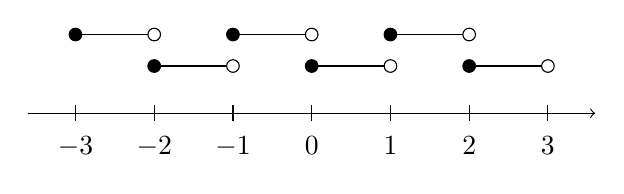
\begin{tikzpicture}
\foreach \i in {-3,-2,-1,0,1,2,3} {
\draw (\i,0.1)--(\i,-0.1) node[below=2pt] {$\i$};
};
\foreach \i in {-3,-1,1} {
 \foreach \j in {0,1} {
  \draw (\i+\j,1-0.4*\j)--(\i+\j+1,1-0.4*\j) ;
  \draw[fill] (\i+\j,1-0.4*\j) circle [radius=0.08] ;
  \draw[fill=white] (\i+\j+1,1-0.4*\j) circle [radius=0.08] ;
};};
\draw[->]  (-3.6,0)--(3.6,0);
\end{tikzpicture}
\end{center}
Clearly, we have $\bigcup_{n=0}^{\infty}[a_n,a_n+1) = \R$. Since, for all $n\in \N$, $[a_n,a_n+1)\in\sigma(\mathcal{O}_{\R})$ and $\lambda\bigl([a_n,a_n+1)\bigr) = 1<\infty$, the Lebesgue measure $\lambda$ is finite.
\eq

This can easily be generalised to show that $\lambda^d$ is finite for all $d\geq 1$.


\subsection{Measurable maps}

As we have remarked earlier, once we introduce a new structure, we should immediately think about the associated structure-preserving maps. In the case of measurable spaces, a measurable map is one that preserves the ``measurability'' structure.

\bd
Let $(M,\Sigma_M)$ and $(N,\Sigma_N)$ be measurable spaces. A map $f\cl M\to N$ is said to be \emph{measurable}\index{measurable map} if
\bse
\forall \, A\in \Sigma_N : \ \preim_f(A)\in \Sigma_M.
\ese
\ed

Note that this is exactly the definition of continuous map between topological spaces, with ``continuous'' replaced by ``measurable'' and topologies replaced by $\sigma$-algebras. 

\bl
Let $(M,\Sigma_M)$ and $(N,\Sigma_N)$ be measurable spaces. A map $f\cl M\to N$ is measurable if, and only if,
\bse
\forall \, A\in \mathcal{E} : \ \preim_f(A)\in \Sigma_M,
\ese
where $\mathcal{E}\subseteq\mathscr{P}(N)$ is a generating set of $\Sigma_N$.
\el

\bc
Let $(M,\mathcal{O}_M)$ and $(N,\mathcal{O}_N)$ be topological spaces. Any continuous map $M\to N$ is measurable with respect to the Borel $\sigma$-algebras on $M$ and $N$.
\ec

Recall that a map $\R\to\R$ is monotonic if it is either increasing or decreasing.

\bc
Any monotonic map $\R\to\R$ is measurable with respect to the Borel $\sigma$-algebra (with respect to $\mathcal{O}_{\R}$).
\ec

\bp
Let $(M,\Sigma_M)$, $(N,\Sigma_N)$ and $(P,\Sigma_P)$ be measurable spaces. If $f\cl M\to N$ and $g\cl N\to P$ are both measurable, the so is their composition $g \circ f\cl M\to P$.
\ep

\bq
Let $A\in \Sigma_P$. As $g$ is measurable, we have $\preim_g(A)\in\Sigma_N$. Then, since $f$ is measurable, it follows that
\bse
\preim_f(\preim_g(A)) = \preim_{g\circ f}(A) \in \Sigma_M.
\ese
Hence, $g\circ f$ is measurable.
\eq

\bp
Let $(M,\Sigma_M)$ and $(N,\Sigma_N)$ be measurable spaces and let $\{f_n\}_{n\in\N}$ be a sequence of measurable maps from $M$ to $N$ whose pointwise limit is $f$. Then, $f$ is measurable.
\ep
Recall that $\{f_n\}_{n\in\N}$ converges pointwise to $f\cl M\to N$ if
\bse
\forall \, m\in M : \ \lim_{n\to \infty}f_n(m)=f(m).
\ese
This is in contrast with continuity, as pointwise convergence of a sequence of continuous maps is not a sufficient condition for the continuity of the pointwise limit. In the case of real or complex-valued maps, a sufficient condition is convergence with respect to the supremum norm. 

\subsection{Push-forward of a measure}

If we have a structure-preserving map $f$ between two instances $A$ and $B$ of some structure, and an object on $A$ (which depends in some way on the structure), we can often use $f$ to induce a similar object on $B$. This is generically called the push-forward of that object along the map $f$.

\bp
Let $(M,\Sigma_M,\mu)$ be a measure space, let $(N,\Sigma_N)$ be a measurable space and let $f\cl M\to N$ be a measurable map. Then, the map
\bi{rrCl}
f_*\mu\cl & \Sigma_N & \to & [0,\infty]\\
& A & \mapsto & \mu(\preim_f(A))
\ei
is a measure on $(N,\Sigma_N)$ called the \emph{push-forward}\index{push-forward of a measure} of $\mu$ along $f$.
\ep

That $f_*\mu$ is a measure follows easily from the fact that $\mu$ is a measure and basic properties of pre-images of maps, namely
\bi{rCl}
\preim_f(A\setminus B) & = & \preim_f(A)\setminus \preim_f(B)\\ \preim_f\biggl(\bigcup_{\,i\in I}A_i\biggr) & = & \bigcup_{i\in I}\preim_f(A_i).
\ei











